\documentclass[a4paper]{report}
\usepackage[brazil]{babel}
\usepackage{graphicx}
\usepackage{imakeidx}
\usepackage{lettrine}
\makeindex[columns=3, title=keywords, intoc]

\title{Verde e Brutall}
\author{el comodin - smvb}
\date{ agosto 2017}

\renewcommand*\contentsname{idx} 

\begin{document}
 
\maketitle
 
\tableofcontents
\clearpage
\addcontentsline{toc}{section}{o verso}
\section*{janela aberta}

\lettrine[findent=2pt]{\fbox{\textbf{E}}}{ }ssa \'e a saga\index{saga} de um encontro com a maquina, escrita por um motorista, e narrada por um autom\'ovel 
fabricado no brasil, desenhado por uma garota, filha de um empresario carioca, que administrou a f\'abrica de
 implementos agricolas e ferroviarios em Entre Rios.

A saga brasilis da injambra e do espirito criativo\index{criativo} aliada a emo\c{c}\~ao

Devido aos diversos acontecimentos, que ao longo do tempo vivenciei, tive a ideia de 
registrar as coisas mais interessantes pois sei que daqui pra frente vai ser cada vez mais dif\'icil algu\'em vicenciar,
tais acontecimentos, tanto pela modernidade e complexidade gradual dos meios de transporte dispon\'iveis, quanto pela propria
natureza humana de querer sempre facilitar, abstrair e se afastar o m\'aximo possivel de saber como as coisas funcionam,
afastando-se, cada vez mais, da aventura e do instinto\index{instinto}.

Pra mim, \'e isso que significa um autom\'ovel antigo, afastar um passo do materialismode querer sempre o carro zero, da moda, da preocupa\c{c}\~ao natural de nossos dias
e aproximar um passo do natural, do divertido, do instinto e de tudo que da gra\c{c}a a vida, a aventura, a emo\c{c}\~ao.

E n\~ao sou o \'unico que pensa assim, vide mujica, grande mestre do nosso tempo que nao me deixa mentir \dots

\'E disso que se trata esse livro, o prazer da vida contado por uma maquina de 6 cilindros\index{6 cilindros}, 4 rodas e um cora\c{c}\~ao.

Agrade\c{c}o a todos os amigos(as) que fizeram parte desta aventura, e desde j\'a dedico esta obra a todos voc\^es.
\clearpage
\addcontentsline{toc}{section}{descoberta}
\section*{A descoberta}
Nos anos 80, quando eu tinha meus 11 anos, havia uma santa matilde\index{santa matilde} branco perolada na minha cidade,
eu passava por ela algumas vezes, indo ou voltando da escola, sempre achei o carro mais bacana de todos\dots

\addcontentsline{toc}{figure}{o sm branco}
\begin{figure}[!htb]
\centering
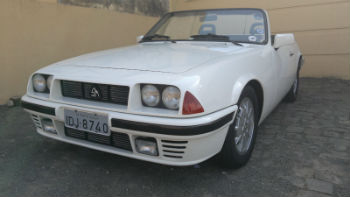
\includegraphics{sm_bco_per}
\caption{SM branco Perolado}
\label{sm_bco}
\end{figure}

Esta id\'eia fortaleceu na minha mente, quando em meados dos 80 o filme "devolta para o futuro" chegou aos cinemas, naturamente como todos nessa \'epoca
fui assistir e como amante de tecnologia e fic\c{c}\~ao fiquei encantado pra n\~ao dizer, abestado por aquele delorean, naturalmente a imagem da SM perolada
voltou para minha cabe\c{c}a como sendo o mais proximo que eu podia achar no brasil de uma. Salvo \'e claro os detalhes t\'ecnicos da viagem no tempo q requer
a lataria exposta para conduzir os 1.21 GigaWats pela superficie permitindo o deslocamento temporal \dots

Certo dia, pela manh\~a, seu Louren\c{c}o, meu falecido pai, me pediu para ligar o carro, um ford scord ghia, para aquecer o motor.

Mesmo n\~ao sendo necess\'ario para um carro relativamente moderno para \'epoca, para mim foi uma experi\^encia \'unica,
at\'e aquele momento, eu nunca havia ligado um carro, pra mim foi um divisor de \'aguas para a vida adulta.

Obviamente eu n\~ao fazia ideia do funcionamento da embreagem e da marcha, liguei o carro com a marcha engatada e por sorte
nao demoli a frente do carro, foi a unica e ultima vez que tive a chance de fazer aquilo, mas a emo\c{c}\~ao do motor ligando ficou
na minha mem\'oria. 

Naquele mesmo ano vi mais algumas vezes a SM branco perolado e pensei que se algum dia eu pudesse ter um
autom\'ovel, seria uma SM, esse dia chegou em 2011.
\clearpage
Eu estava visitando uns amigos em rio grande e fui convidado para almo\c{c}ar \`a bordo com a tripula\c{c}\~ao do Atl\~antico Sul.

\addcontentsline{toc}{figure}{atl\^antico Sul}
\begin{figure}[!htb]
\centering
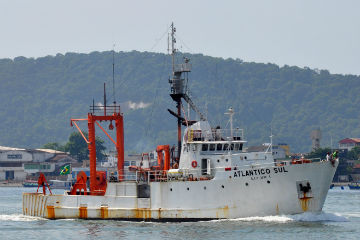
\includegraphics{atsul}
\caption{Navio oceanogr\'afico da FURG}
\label{at_sul}
\end{figure}

Durante o almo\c{c}o o assunto se dirigiu para autom\'oveis, lembrei do meu antigo sonho e compartilhei com o pessoal, nesta ocasi\~ao um dos marinheiros
me falou que havia uma santa matilde a venda em tapes, um conhecido.

Meu amigo Stefan, que havia convidado para o almo\c{c}o com sua equipe de trabalho, entusiamou-se com a informa\c{c}\~ao, e eu tambem, obviamente, e na semana 
seguinte fomos com mais um amigo de rio grande, Daniel Torres, vulgo "bala", outro entusiasta dos 6cilindros, ver a preciosidade.

Durante o trajeto, rio grande - tapes, conversamos muito, sobre os motores, a divers\~ao, pescarias, mas o que nao saia da cabe\c{c}a, a SM.   
\clearpage
\addcontentsline{toc}{section}{primeira vinda}
\section*{primeira vinda}

Era verde, assim como seu interior, perfeita, parecia tudo ok quando vimos, exceto os pneus, esses estavam na capa da gaita

\addcontentsline{toc}{figure}{273a sm}
\begin{figure}[!htb]
\centering
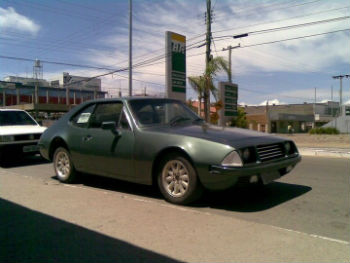
\includegraphics{sm273}
\caption{273$^{a}$SM -fonte: Cadastro Nacional da Santa Matilde}
\label{sm_273}
\end{figure}

\addcontentsline{toc}{section}{TODO}
\section*{prot\'otipo e ideias soltas}
Uma coisa que eu notei \'e q me senti livre para criar pois sabendo como funciona eu facilmente posso adaptar algo e nao ficar na m\~ao
\clearpage
\printindex
\end{document}
